\chapter{Runtime View (Dynamic View)}

\section{System Initialization}
\label{sec:System_Initialization}

\Requirement{003}
{
The initialization runnable entity Runnable_DIAG_Init is responsible for initializing all variables and state machines.
}
{\Satisfies{SRS_DIAG 084} \Satisfies{SRS_DIAG 060}}

\input{generated/tables/Runnable_DIAG_Init.tex}

\Requirement{081}
{
If the configuration parameter DiagGenerateInitRunnable is TRUE the Runnable_DIAG_Init calls the DIAG initiation function only once, otherwise the user shall call the function DIAG_Init in the BswM initialization action list.
}
{\Satisfies{SRS_DIAG 106}}

\section{System de-initialization}

\Requirement{004}
{
SUM_DIAG shall implement the ShutdownPermission interface to SUM_SUSD to indicate whether it has enabled shutdown. The shutdown is NOT enabled if there is any UDS request ongoing or the current Session is not DEFAULT, unless an ECU Reset has been requested via the PermitExecution interface (bit 6 cleared), in which case shutdown is enabled regardless of session.
}
{\Satisfies{SRS_DIAG 082} \Satisfies{SRS_DIAG 119} \Satisfies{SRS_DIAG 120} \Satisfies{SRS_DIAG 121}}

\Requirement{066}
{
SUM_DIAG shall also implement an aliveness mechanism to notify SUM_SUSD of its functioning status
}
{\Satisfies{SRS_DIAG 083}}

\Requirement{005}
{
SUM_DIAG shall update the corresponding signal at a project specific period with a rolling count updated value. SUM_DIAG shall notify SUM_SUSD with the shutdown value when the shutdown permission state is reached.
}
{\Satisfies{SRS_DIAG 099}}

\input{generated/tables/Runnable_Shutdown_Permission.tex}

\begin{figure}[h]
	\centering
		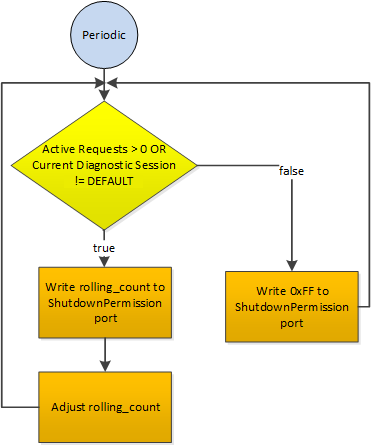
\includegraphics[width=8cm]{images/Runnable_Shutdown_Permission_diagram}
	\caption{Runnable_Shutdown_Permission diagram}
\end{figure}

\section{Private Function}

The following private functions are implemented in the source file SUM_DIAG.c.


\subsection{initializeForRun}

\Requirement{007}
{
\input{generated/tables/initializeForRun.tex}
}
{\Satisfies{SRS_DIAG 006} \Satisfies{SRS_DIAG 007} \Satisfies{SRS_DIAG 008} \Satisfies{SRS_DIAG 009} \Satisfies{SRS_DIAG 012} \Satisfies{SRS_DIAG 016}}

\subsection{setTesterAddress}

\Requirement{008}
{
\input{generated/tables/setTesterAddress.tex}
}
{\Satisfies{SRS_DIAG 014}}

\subsection{getTesterAddress}

\Requirement{009}
{
\input{generated/tables/getTesterAddress.tex}
}
{\Satisfies{SRS_DIAG 014}}

\subsection{setManufacturerEnableCounter}

\Requirement{010}
{
\input{generated/tables/setManufacturerEnableCounter.tex}
}
{\Satisfies{SRS_DIAG 006}}

\subsection{getManufacturerEnableCounter}

\Requirement{011}
{
\input{generated/tables/getManufacturerEnableCounter.tex}
}
{\Satisfies{SRS_DIAG 006}}

\subsection{getEcuAddress}

\Requirement{012}
{
\input{generated/tables/getEcuAddress.tex}
}
{\Satisfies{SRS_DIAG 019}}

\subsection{setOtaPsf}

\Requirement{013}
{
\input{generated/tables/setOtaPsf.tex}
}
{\Satisfies{SRS_DIAG 095} \Satisfies{SRS_DIAG 124}}

\subsection{getOtaPsf}

\Requirement{014}
{
\input{generated/tables/getOtaPsf.tex}
}
{\Satisfies{SRS_DIAG 095}}

\subsection{check_offpowermode}

\Requirement{016}
{
\input{generated/tables/check_offpowermode.tex}
}
{\Satisfies{SRS_DIAG 013}}

\section{Function related to DCM callout}

\subsection{Diag_SetProgConditions}
\label{subsec:Diag_SetProgConditions}

\Requirement{017}
{
\input{generated/tables/Diag_SetProgConditions.tex}
}
{\Satisfies{SRS_DIAG 093}}

\subsection{SUM\_DIAG\_DcmGetRxPermission}
\label{subsec:DIAG_DcmGetRxPermission}

\Requirement{117}
{
The SUM\_DIAG\_DcmGetRxPermission callout shall perform enable-condition checks for protocol pre-emption by validating the protocol type, PDU ID, tester source address, and vehicle power mode. The callout shall return E\_OK only when all enable conditions are satisfied; otherwise it shall return E\_NOT\_OK.
}
{\Satisfies{SRS_DIAG 122} \Satisfies{SRS_DIAG 123}}

\Requirement{118}
{
SUM\_DIAG\_DcmGetRxPermission shall support the protocol types defined for pre-emption (OBDonUDS, OBDS0aD, ZEVonUDS on CAN or ETH), restrict tester source addresses to the configured list (for example 0x0E00), and block pre-emption if vehicle power mode is OFF or the protocol/tester source address is invalid.
}
{\Satisfies{SRS_DIAG 122} \Satisfies{SRS_DIAG 123}}

\section{Data design}

\subsection{MACRO Definitions}
\label{subsec:macro}

\Macro{DIAG_MIN_ROLLING_COUNT}
{0u}
{Minimum shutdown rolling count}

\Macro{DIAG_MAX_ROLLING_COUNT}
{3u}
{Maximum shutdown rolling count}

\Macro{DIAG_ENABLE_SHUTDOWN}
{0xFF}
{Permit shutdown for PermitShutdown interface}

\Macro{DIAG_START_OF_CYCLE}
{0u}
{Start of ECU Operating mode sleep -normal operation – sleep cycle}

\Macro{DIAG_SLEEP2}
{1u}
{Sleep mode after normal operation mode}

\Macro{DIAG_NORMAL_OPERATION}
{2u}
{Normal operation mode}

\Macro{PHYSICAL_REQUEST}
{0u}
{Diagnostic Physical Request type}

\Macro{FUNCTIONAL_REQUEST}
{1u}
{Diagnostic Functional Request type}

\Macro{IDX_SUBFUNCTION}
{0u}
{RequestData index for sub function}

\Macro{IDX_SUBFUNCTION_IO}
{2u}
{UDS spec for SIDs with sub functions}

\Macro{DIAG_SESSION_CTRL_MIN_DATASIZE}
{1u}
{Minimum RequestData data size for DiagnosticSessionControl request}

\Macro{ECU_RESET_MIN_DATASIZE}
{1u}
{Minimum RequestData data size for EcuReset request}

\Macro{COMM_CTRL_MIN_DATASIZE}
{1u}
{Minimum RequestData data size for CommunicationControl request}

\Macro{DYN_DEFINE_DATA_ID_MIN_DATASIZE}
{3u}
{Minimum RequestData data size for DynamicallyDefineDataIdentifier request}

\Macro{RMBA_SERVICE_SUPPORT}
{1u}
{Used to check if ECU supports Read Memory by Address service of DCM}

\Macro{TESTER_FROM_SOURCE}
{N/A}
{Macro for reading Tester Source Address from source address}

\Macro{MEC_INITIAL_VALUE}
{read from configuration}
{Initial value for Manufacturing Enable Counter}

\section{Type Definitions}

\subsection{UDSDiagnosticServiceIds}

\Requirement{018}
{
\input{generated/tables/UDSDiagnosticServiceIds.tex}
}
{\Satisfies{SRS_DIAG 004}\Satisfies{SRS_DIAG 101}}

\subsection{SubFunctions}

\Requirement{019}
{
\input{generated/tables/SubFunctions.tex}
}
{\Satisfies{SRS_DIAG 004}\Satisfies{SRS_DIAG 101}}

\subsection{Diag_NormalCommStatus_Channel_Type}

\Requirement{021}
{
\input{generated/tables/Diag_NormalCommStatus_Channel_Type.tex}
}
{\Satisfies{SRS_DIAG 016}}

\section{Wake up procedure}

\section{Sleep procedure}

\section{Boot loading procedure}

\section{Failure handling strategy}

\section{Critical timing constraints}

\section{Tasks management}
\label{sec:Tasks_management}

\subsection{Periodic Runnables}
\label{subsec:Periodic_Run}
The following periodic runnables and the event-triggered runnables are implemented in the source file SUM_DIAG_Runnables.c, while the Indication and Confirmation routines are implemented in the source file SUM_DIAG_Services.c.

\subsubsection{Runnable_DIAG_Init}
{
Described in section \ref{sec:System_Initialization}.
}
\subsubsection{Runnable_DIAG_Main}
\label{subsec:Runnable_DIAG_Main}
\Requirement{022}
{
SUM_DIAG shall implement a port, PermitExecution, which receives a notification from SUM_SUSD whether it should execute its functions. 
}
{\Satisfies{SRS_DIAG 007}}
SUM_DIAG shall start the execution of its functions when the Wakeup(s) Active bit (Bus relevant) in the SUSD_DIAG_PermitExecution interface is TRUE.\newline
{\Satisfies{SRS_DIAG 008}}

\input{generated/tables/Runnable_DIAG_Main.tex}

\subsubsection{Runnable_BswM_ ModeUser}

\Requirement{023}
{
Runnable_BswM_ModeUser shall notify SSM module of communication mode status.
}
{\Satisfies{SRS_DIAG 079}}

\Requirement{024}
{
Runnable_BswM_ModeUser shall receive the Normal Communications type from Dcm.
}
{\Satisfies{SRS_DIAG 016}}

\Requirement{025}
{
Runnable_BswM_ModeUser shall receive the session control type from Dcm.
}
{\Satisfies{SRS_DIAG 017}}

\input{generated/tables/Runnable_BswM_ModeUser.tex}

\subsubsection{Runnable_MEC_Handler}

\Requirement{026}
{
Runnable_MEC_Handler is responsible to decrement the MEC value by one count upon each vehicle ignition cycle.
}
{\Satisfies{SRS_DIAG 073}}

\Requirement{072}
{
It is also responsible to write the updated value into NvM by validating the RAM block and output MEC when a change has occurred
}
{\Satisfies{SRS_DIAG 066}}

\Requirement{104}
{
To ensure a successful write of the MEC value into the NVM, the DIAG verifies that the battery voltage condition is met using the BatteryVoltage_DisableNVMWrite port interface provided by the SUSD module. 
}
{\Satisfies{SRS_DIAG 110}}

\Requirement{027}
{
Once the MEC value reaches 0 it shall be ignored and not be written to the NvM
}
{\Satisfies{SRS_DIAG 078}}

\input{generated/tables/Runnable_MEC_Handler.tex}

\begin{figure}[h]
	\centering
		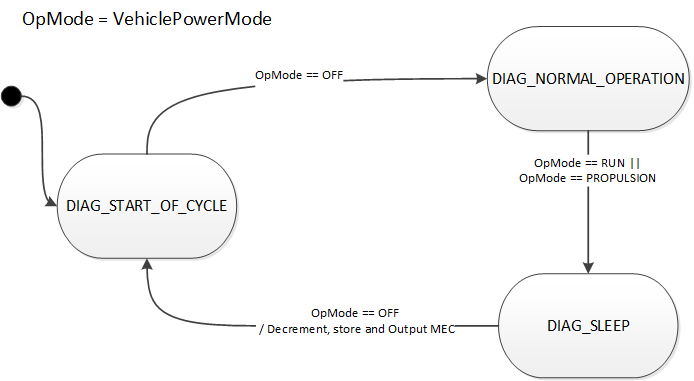
\includegraphics{images/MEC_Handler_state_diagram}
	\caption{MEC Handler state diagram}
\end{figure}

\subsubsection{Runnable_OTA_PSF}
\label{subsec:Re_Otapsf}

\Requirement{035}
{
The SUM_DIAG module receives the Remote Programming Active Authenticated network signal from the Com, after receiving the fault active and availability status of this signal from the SUM_SSFM-SSM module.
The reception of the network signal allows the module to receive, calculate and supply the OTA_PSF value.
}
{\Satisfies{SRS_DIAG 112} \Satisfies{SRS_DIAG 113} \Satisfies{SRS_DIAG 122}}

\Requirement{028}
{
The SUM_DIAG module shall SET or CLEAR the OTA_PSF value based on the network signal received and also taking into account whether the ECU's internal conditions are favorable to support the OTA programming session transition. 
}
{\Satisfies{SRS_DIAG 094} \Satisfies{SRS_DIAG 114} \Satisfies{SRS_DIAG 124}}

\Requirement{029}
{
The module shall store the OTA_PSF in NvM or Flash Emulated EEPROM to ensure its value is not lost upon sleep, shutdown, reset or loss of power.
}
{\Satisfies{SRS_DIAG 095}}

\Requirement{103}
{To ensure a successful write of the OTA_PSF into the NVM, the DIAG verifies that the battery voltage condition is met using the BatteryVoltage_DisableNVMWrite port interface provided by the SUSD module. 
}
{\Satisfies{SRS_DIAG 110}}

\Requirement{030}
{
When OTA_PSF is SET, the ECU shall Set the EnableCondition-OTAPSF to FALSE. 
}
{\Satisfies{SRS_DIAG 096}}

\Requirement{031}
{
When OTA_PSF is CLEARED, the ECU shall SET the EnableCondition-OTAPSF to TRUE.
}
{\Satisfies{SRS_DIAG 097}}


\Requirement{032}
{
A periodic runnable shall be implemented to implement Automatic Disabling of DTCs when OTA_PSF is SET in in-vehicle ECUs.
}
{\Satisfies{SRS_DIAG 061} \Satisfies{SRS_DIAG 010} \Satisfies{SRS_DIAG 109}}


\input{generated/tables/Runnable_OTA_PSF.tex}

\subsection{Event-Triggered Runnables}
\label{subsec:Event-Triggered_runnables}

\subsubsection{DCM ControlDTCSetting}
\label{subsubsec:DCM_ControlDTCSetting}
The SUM\_DIAG needs to know the ControlDTCSetting information from the DCM and receives it through the mode switch interface of the BswM module. 
To handle the ControlDTCSetting information sent by the DCM, the SUM\_DIAG has two runnables.
Runnable\_DIAG\_ControlDTCSetting\_Enabled and Runnable\_DIAG\_ControlDTCSetting\_Disabled,
which are triggered with one of the two modes of the SUM\_ControlDTCSetting interface (ControlDTCSetting Enabled/Disabled).

\Requirement{006}
{
\input{generated/tables/Runnable_DIAG_ControlDTCSetting_Disabled.tex}
\input{generated/tables/Runnable_DIAG_ControlDTCSetting_Enabled.tex}
}
{\Satisfies{SRS_DIAG 027} \Satisfies{SRS_DIAG 111} \Satisfies{SRS_DIAG 124}}

\Requirement{033}
{
Runnable_RequestHandler_Indication and Runnable_ RequestHandler_Confirmation implement algorithms needed to support diagnostic service requests.
}
{\Satisfies{SRS_DIAG 011}}
\Requirement{034}
{
Runnable Indications shall implement the pre-condition checks for the listed diagnostic service requests. 
}
{\Satisfies{SRS_DIAG 004}}

\subsubsection{Runnable_RequestHandler_Indication}

\input{generated/tables/Runnable_RequestHandler_Indication.tex}
 \clearpage
 
\begin{figure}[h]
	\centering
		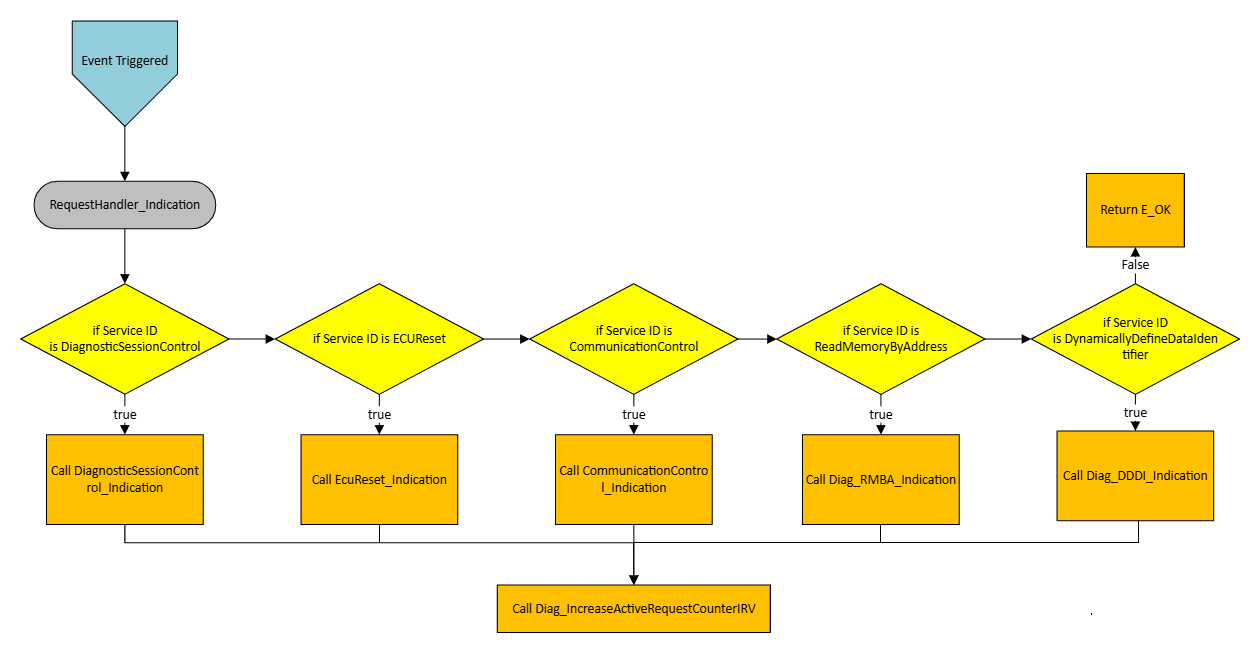
\includegraphics[width=16cm]{images/Runnable_RequestHandler_Indication_diagram}
	\caption{Runnable_RequestHandler_Indication diagram}
\end{figure}

\subsubsection{Runnable_RequestHandler_Confirmation}

\input{generated/tables/Runnable_RequestHandler_Confirmation.tex}

\begin{figure}[h]
	\centering
		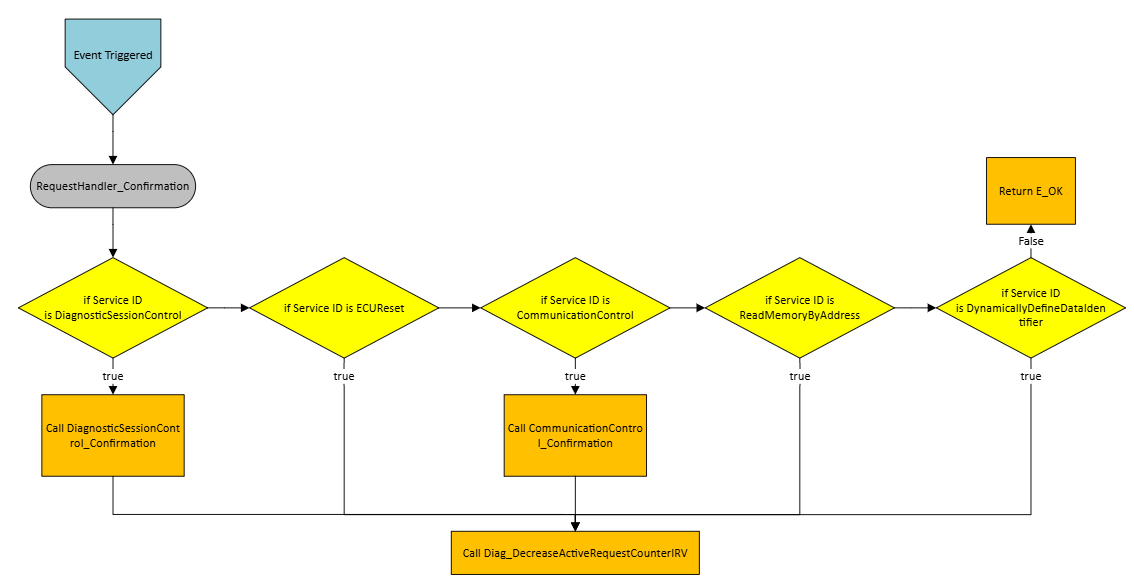
\includegraphics[width=16cm]{images/Runnable_RequestHandler_Confirmation_diagram}
	\caption{Runnable_RequestHandler_Confirmation diagram}
\end{figure}

\subsubsection{Indication and Confirmation Routines}

\Requirement{036}
{
Indication routines, when necessary, shall get the vehicle power mode from the SUSD module to determine Off_power_mode status.
}
{\Satisfies{SRS_DIAG 013}}

\Requirement{039}
{
Confirmation routines, when necessary, shall store the Tester Source address. 1 and 2 byte Tester Source addresses, for CAN and ETH respectively, shall be supported. 
}
{\Satisfies{SRS_DIAG 014} \Satisfies{SRS_DIAG 124} \Satisfies{SRS_DIAG 125}}

\Requirement{040}
{
Confirmation routines, when necessary, shall store the Tester Address using the function Diag_SetProgConditions ().
}
{\Satisfies{SRS_DIAG 093}}

\subsubsection{CommunicationControl_Indication}
\label{subsec:communicationControl}

\Requirement{041}
{
CommunicationControl_Indication implements the Indication function needed for pre-condition checks of CommunicationControl diagnostic requests.
}
{\Satisfies{SRS_DIAG 045}}

\Requirement{042}
{
CommunicationControl_Indication shall accept request for Sub-Function 0x00.
}
{\Satisfies{SRS_DIAG 087} \Satisfies{SRS_DIAG 045}}

\Requirement{043}
{
CommunicationControl_Indication shall accept request for Sub-Function 0x03 if power mode is OFF, otherwise NRC 0x22 will be returned.
}
{\Satisfies{SRS_DIAG 087} \Satisfies{SRS_DIAG 088} \Satisfies{SRS_DIAG 045}}

\Requirement{044}
{
CommunicationControl_Indication shall not accept request for Sub-Functions other than 0x00 or 0x03.
}
{\Satisfies{SRS_DIAG 045}}

\input{generated/tables/CommunicationControl_Indication.tex}

\begin{figure}[H]
	\centering
		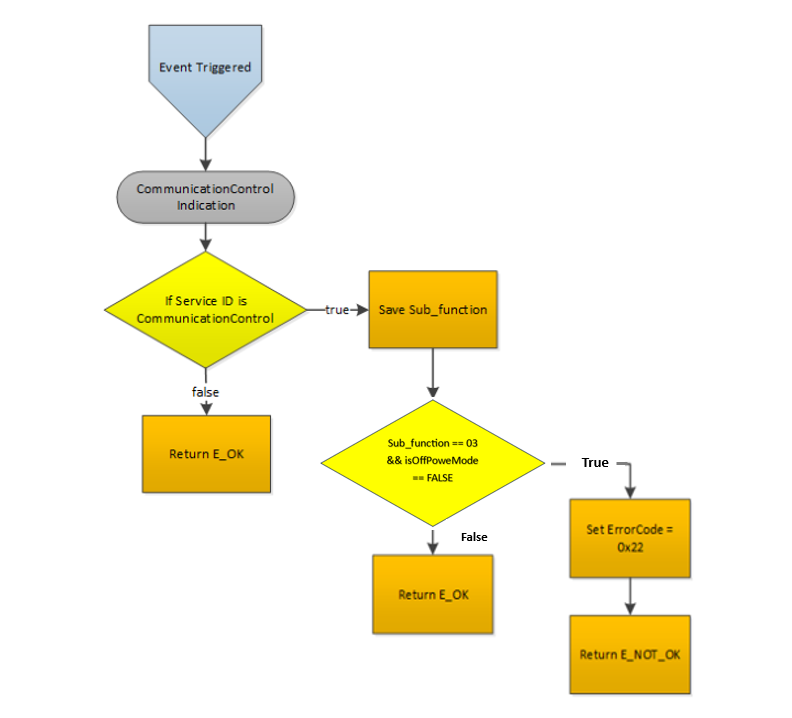
\includegraphics[width=13.5cm]{images/CommunicationControl_Indication_diagram}
	\caption{CommunicationControl_Indication diagram}
\end{figure}

\subsubsection{CommunicationControl_Confirmation}

\Requirement{045}
{
CommunicationControl_Confirmation implements the Confirmation function needed for CommunicationControl diagnostic request to store tester source address and set normal_msg_transmission flag.
}
{\Satisfies{SRS_DIAG 047} \Satisfies{SRS_DIAG 124}}

\input{generated/tables/CommunicationControl_Confirmation.tex}

\begin{figure}[H]
	\centering
		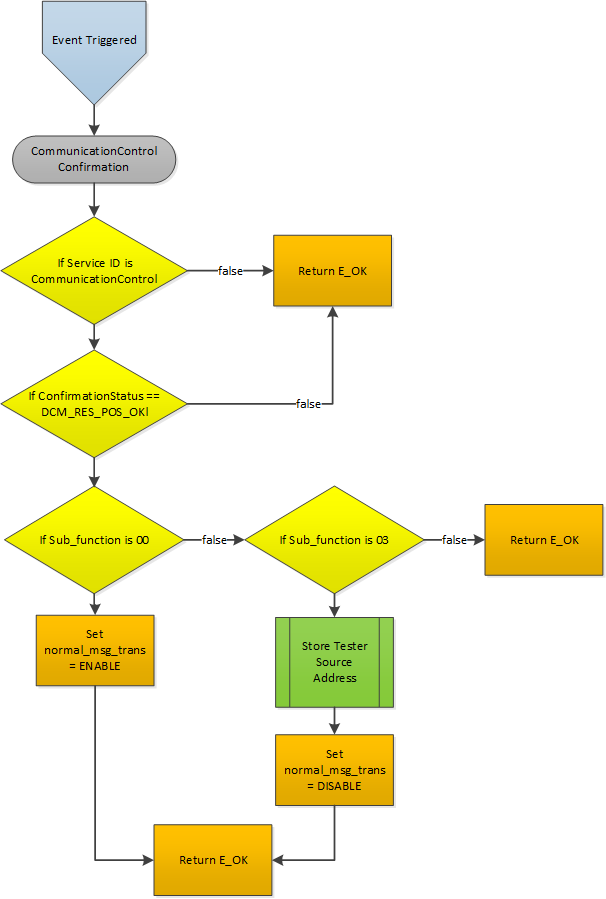
\includegraphics[width=11.5cm]{images/CommunicationControl_Confirmation_diagram}
	\caption{CommunicationControl_Confirmation diagram}
\end{figure}

\subsubsection{DiagnosticSessionControl_Indication}

\Requirement{046}
{
DiagnosticSessionControl_Indication implements the Indication function needed for pre-condition checks of DiagnosticSessionControl diagnostic requests.
}
{\Satisfies{SRS_DIAG 027}}

\Requirement{047}
{
DiagnosticSessionControl_Indication shall accept request for Sub-Function 0x02 if normal_msg_transmission is disabled, DTC setting is disabled and Power mode is OFF, else NRC 0x22 is returned. It shall ignore the suppressPosRspMsgIndicationBit of the Sub-Function received.
}
{\Satisfies{SRS_DIAG 085}}

\Requirement{080}
{
SUM_DIAG will notify whether the DiagnosticSessionControl – Programming Session request took place to SUM_SOH through interface DIAG_SOH_DiagSessionRequest.
}
{\Satisfies{SRS_DIAG 103}}

\Requirement{049}
{
All the ECU specific preconditions for change to programming session request shall be verified in ECU specific SW-C by configuring supplier specific ServiceRequestNotification interface.
}
{\Satisfies{SRS_DIAG 098}}

\input{generated/tables/DiagnosticSessionControl_Indication.tex}

\begin{figure}[H]
	\centering
		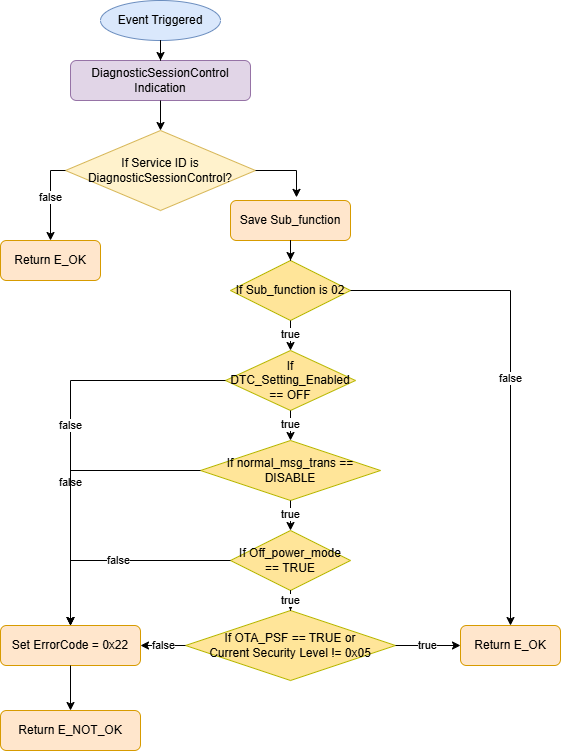
\includegraphics[width=13cm]{images/DiagnosticSessionControl_Indication_diagram}
	\caption{DiagnosticSessionControl_Indication diagram}
\end{figure}

\subsection{Diag_IncreaseActiveRequestCounterIRV}

\Requirement{115}
{
\input{generated/tables/Diag_IncreaseActiveRequestCounterIRV.tex}
}
{\Satisfies{SRS_DIAG 119} \Satisfies{SRS_DIAG 121}}

\subsubsection{DiagnosticSessionControl_Confirmation}

\Requirement{050}
{
DiagnosticSessionControl_Confirmation implements the Confirmation function needed for DiagnosticSessionControl diagnostic request to store tester source address and reset flags.
}
{\Satisfies{SRS_DIAG 028} \Satisfies{SRS_DIAG 124}}

\input{generated/tables/DiagnosticSessionControl_Confirmation.tex}
\clearpage

\begin{figure}[H]
	\centering
		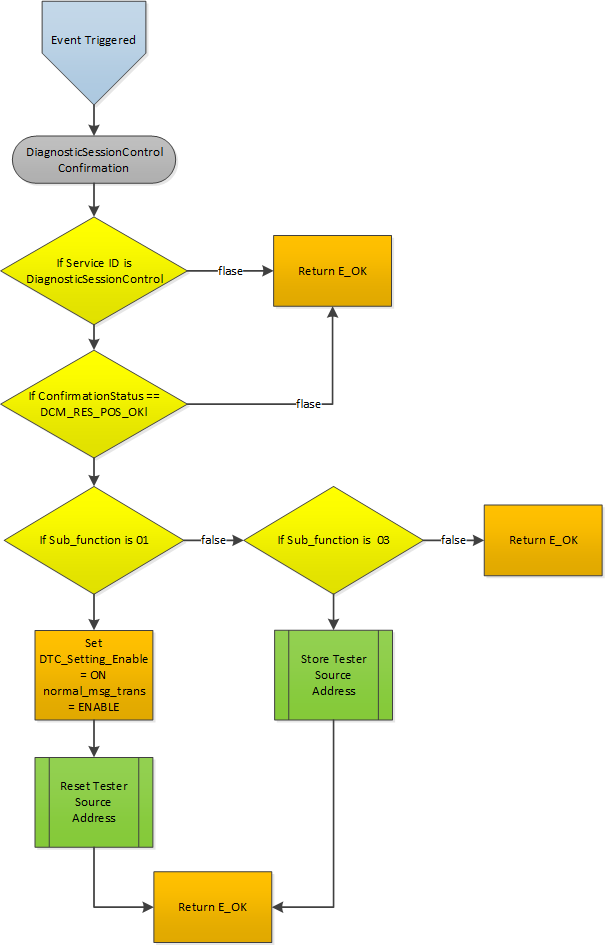
\includegraphics[width=13cm]{images/DiagnosticSessionControl_Confirmation_diagram}
	\caption{DiagnosticSessionControl_Confirmation diagram}
\end{figure}

\subsubsection{DynamicallyDefineDataIdentifier_Indication}
\label{subsec:DDDI}

\Requirement{051}
{
DynamicallyDefineDataIdentifier_Indication implements the Indication function needed for pre-condition checks of DynamicallyDefineDataIdentifier diagnostic requests.
}
{\Satisfies{SRS_DIAG 054} \Satisfies{SRS_DIAG 055}}
\Requirement{052}
{
DynamicallyDefineDataIdentifier_Indication shall accept request for Sub-Function 0x02 if ReadMemory_Security_Verification () returns E_OK, else NRC 0x31 is returned. It shall ignore the suppressPosRspMsgIndicationBit of the Sub-Function received.
}
{\Satisfies{SRS_DIAG 092}}
\Requirement{075}
{
DynamicallyDefineDataIdentifier_Indication shall be provided to the user only when the configuration parameter DDDI_Support is set to true.
}
{\Satisfies{SRS_DIAG 102} \Satisfies{SRS_DIAG 103}}

\input{generated/tables/DynamicallyDefineDataIdentifier_Indication.tex}

\begin{figure}[H]
	\centering
		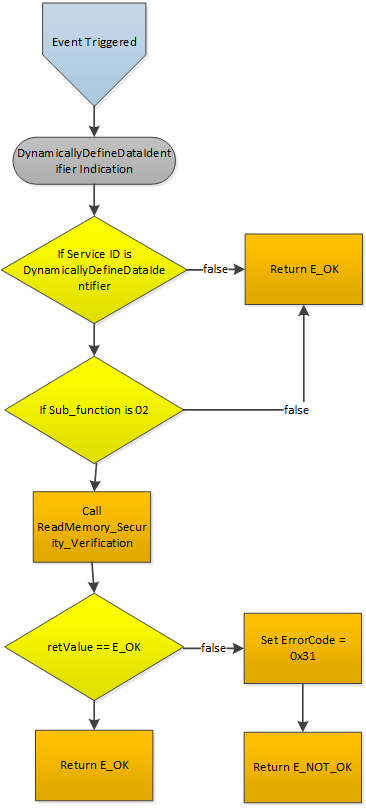
\includegraphics[width=8cm]{images/DynamicallyDefineDataIdentifier_Indication_diagram}
	\caption{DynamicallyDefineDataIdentifier_Indication diagram}
\end{figure}

\subsubsection{EcuReset_Indication}

\Requirement{053}
{
EcuReset_Indication implements the Indication function needed for pre-condition checks of EcuReset diagnostic requests.
}
{\Satisfies{SRS_DIAG 031}}
\Requirement{054}
{
EcuReset_Indication shall accept request for Sub-Function 0x01 if Power mode is OFF, else NRC 0x22 is returned. It shall ignore the suppressPosRspMsgIndicationBit of the Sub-Function received.
}
{\Satisfies{SRS_DIAG 086}}
\Requirement{055}
{
EcuReset_Indication shall receive the reset type from Dcm.
}
{\Satisfies{SRS_DIAG 018}}
\Requirement{056}
{
EcuReset_Indication shall notify the SOH module that an ECU Reset request has been received.
}
{\Satisfies{SRS_DIAG 012}}

\input{generated/tables/EcuReset_Indication.tex}

\begin{figure}[H]
	\centering
		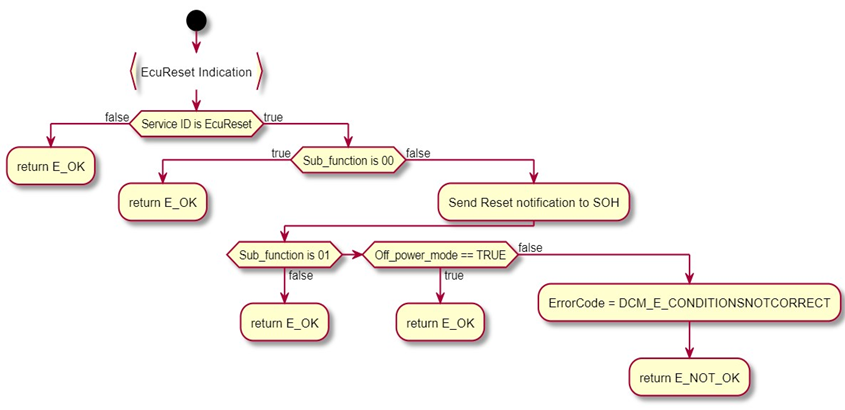
\includegraphics[width=16cm]{images/EcuReset_Indication_diagram}
	\caption{EcuReset_Indication diagram}
\end{figure}

\subsubsection{ReadMemorybyAddress_Indication}
\label{subsec:RMBA}
\Requirement{057}
{
ReadMemorybyAddress_Indication implements the Indication function needed for pre-condition checks of ReadMemoryByAddress diagnostic requests.
}
{\Satisfies{SRS_DIAG 039}}
\Requirement{058}
{
ReadMemorybyAddress_Indication accepts the request only if the request type is physical, otherwise NRC 0x22 (Conditions Not Correct) is sent.
}
{\Satisfies{SRS_DIAG 090}}
\Requirement{073}
{
ReadMemorybyAddress_Indication shall extract the memory address and memory size from the RequestData.
}
{\Satisfies{SRS_DIAG 100}}
\Requirement{059}
{
ReadMemorybyAddress_Indication accepts the request if ReadMemory_Security_Verification () returns E_OK, otherwise NRC 0x31 (Request Out Of Range) is sent.
}
{\Satisfies{SRS_DIAG 091}}
\Requirement{077}
{
ReadMemorybyAddress_Indication shall be provided to the user only when the configuration parameter RMBA_Support is set to true.
}
{\Satisfies{SRS_DIAG 102} \Satisfies{SRS_DIAG 103}}

\input{generated/tables/ReadMemorybyAddress_Indication.tex}
\clearpage

\begin{figure}[H]
	\centering
		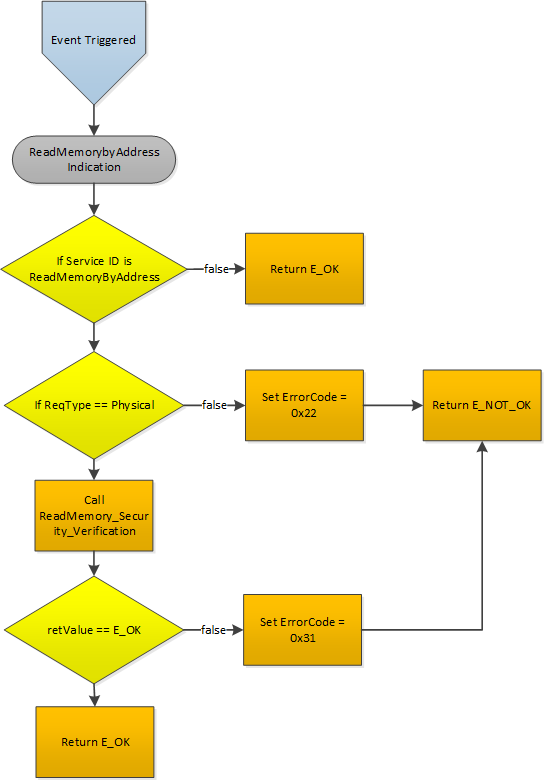
\includegraphics[width=12cm]{images/ReadMemorybyAddress_Indication_diagram}
	\caption{ReadMemorybyAddress_Indication diagram}
\end{figure}

\subsection{Diag_DecreaseActiveRequestCounterIRV}

\Requirement{116}
{
\input{generated/tables/Diag_DecreaseActiveRequestCounterIRV.tex}
}
{\Satisfies{SRS_DIAG 119} \Satisfies{SRS_DIAG 121}}

\subsubsection{WriteData}
\label{subsec:WriteData}
\Requirement{063}
{
This function is responsible for updating MEC data to MEC RAM mirror block when it receives WriteDataByIdentifier service with DID associated with MEC.
}
{\Satisfies{SRS_DIAG 002}}
\Requirement{105}
{
	To ensure a successful write of the MEC value into the NVM, the DIAG verifies that the battery voltage condition is met using the BatteryVoltage_DisableNVMWrite port interface provided by the SUSD module. 

	\input{generated/tables/WriteData.tex}
}
{\Satisfies{SRS_DIAG 110} \Satisfies{SRS_DIAG 064} \Satisfies{SRS_DIAG 065} \Satisfies{SRS_DIAG 074} \Satisfies{SRS_DIAG 078} \Satisfies{SRS_DIAG 080}}

\begin{figure}[H]
	\centering
		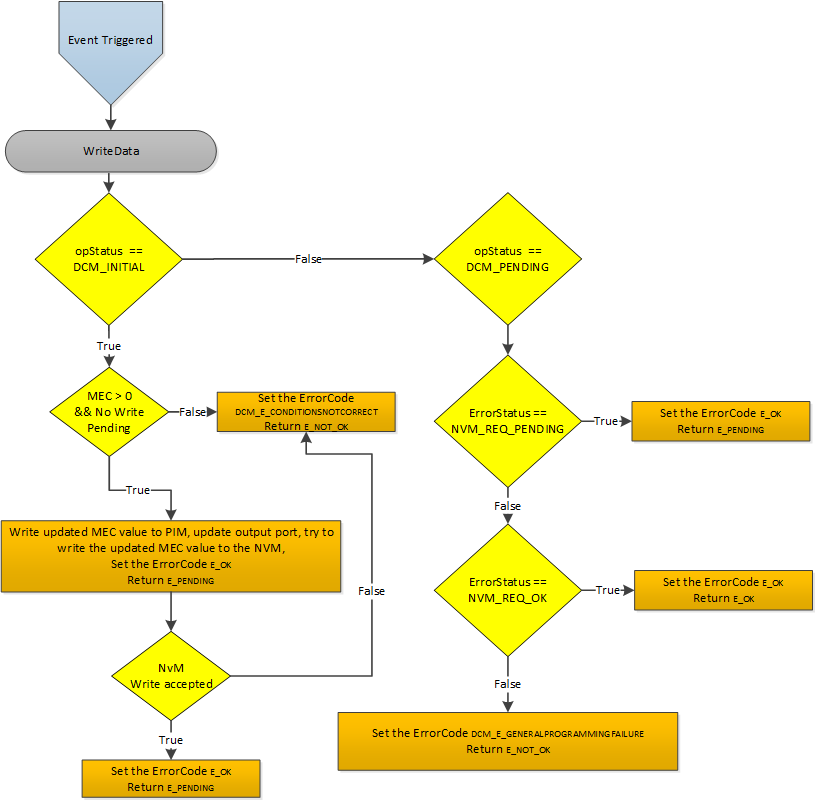
\includegraphics[width=17cm]{images/WriteData_diagram}
	\caption{WriteData diagram}
\end{figure}

\subsubsection{ReadData}

\Requirement{064}
{
This function is responsible for reading the updated MEC data when it receives ReadDataByIdentifier service with DID associated with MEC.
}
{\Satisfies{SRS_DIAG 002} \Satisfies{SRS_DIAG 074} \Satisfies{SRS_DIAG 080}}

\input{generated/tables/ReadData.tex}

\subsubsection{ConditionCheckRead}

\Requirement{065}
{
This function is responsible for checking if the conditions to read the DID associated with the MEC are correct.
}
{\Satisfies{SRS_DIAG 002} \Satisfies{SRS_DIAG 074} \Satisfies{SRS_DIAG 080}}

\input{generated/tables/ConditionCheckRead.tex}

\subsubsection{Runnable_SwitchedToDefaultSession}

\Requirement{083}
{
\input{generated/tables/Runnable_SwitchedToDefaultSession.tex}
}
{\Satisfies{SRS_DIAG 107}}

\subsubsection{Runnable_DID_F1B0_ReadData}
\label{subsubsec:Runnable_DID_F1B0_ReadData}

\Requirement{108}
{
SUM_DIAG shall implement the Runnable_DID_F1B0_ReadData function to handle ReadData requests for DID 0xF1B0. The DID 0xF1B0 is used to read the ECU Address.
}
{\Satisfies{SRS_DIAG 115} \Satisfies{SRS_DIAG 116} \Satisfies{SRS_DIAG 117}}

\subsubsection{Runnable_Diag_DID_E0CC_ReadData}
\label{subsubsec:Runnable_Diag_DID_E0CC_ReadData}

\Requirement{122}
{
The Runnable_Diag_DID_E0CC_ReadData is generated when the parameter Sum_Diag_EnableDID_0xE0CC is enabled to handle ReadData requests for DID 0xE0CC. The function will always return 0x5 (Not supported), which means that the ECU is CAN only and does not have the SrvcMgr.
}
{\Satisfies{SRS_DIAG 126} \Satisfies{SRS_DIAG 127}}

\section{Runtime Scenario} 

\clearpage
